% ***********************************
% Digitális technika 2. jegyzet
% Utolsó frissítés: 2017. május 18.
% vik.wiki-re szánt változat
% Sebők Bence - sebokbence@sch.bme.hu
% ***********************************

\documentclass{article}
\usepackage[utf8]{inputenc} % magyar karakterek
\usepackage{hyperref} % url-ekhez
\usepackage{graphicx} % képekhez
\graphicspath{{./images/}} % melyik mappában vannak a képek
\usepackage{listings} % kódrészletekhez
\lstset{language=[x86masm]Assembler} % kódrészlet színezéséhez
\usepackage{tcolorbox} % szöveg háttérszínéhez

\begin{document}

% címoldal tartalma
\title{Digitális technika 2. jegyzet}
\author{Sebők Bence}
\date{2017. tavasz}

% címoldal generálása
\maketitle

% toc átnevezése
\renewcommand{\contentsname}{Tartalomjegyzék}
% tartalomjegyzék
\tableofcontents

\newpage % új oldal

% jogászkodás
\section{Bevezetés}
Ez a jegyzet a BME Digitális technika 2. tantárgyhoz szeretne segítséget nyújtani. Ezen kezdeményezés célja, hogy segítsen a hallgatóknak megérteni a tananyagot. A tantárgy nehéz, erősen ajánlott előadásra, gyakorlatra járni. Ez a jegyzet csak az előadáson, gyakorlaton készült jegyzet mellé jelent segítséget, nem tanít meg a nulláról a tantárgy minden apróságára.

Ez egy hallgatói jegyzet, nincs lektorálva, se egyetemi oktató által felügyelve. Amit itt olvasol, azt csak saját felelősségre használd, hivatalos helyeken nem hivatkozási alap ez a jegyzet.

\newpage % új oldal

\section{Alapismeretek}
\subsection{Intel 8085 processzor}
\begin{itemize}
	\item PC (Program Counter, program számláló): regisztárpár, ami az aktuálisan használt memóriacímet tartalmazza.
	\item SP (Stack Pointer, stack mutató): a stack tetejére mutató pointer (regiszterpárban tárolja ezt a 2 bájtos címet)
\end{itemize}
%Belső regiszterek:
%\begin{enumerate}
%	\item A (Accumulator): aritmetikai és logikai műveletekhez vannak speciális utasítások, amik az akksit használják.
%	\item F (Flags): az utasítások által állított flag-ekkel tudjuk nyomon követni a rendszer aktuális állapotát.
%\end{enumerate}

\section{Assembly}
Digitális technika 2. tantárgy során az Intel 8085 processzor programozásához használt Assembly programozási nyelvet tanítják. Ez a fejezet erről az Assembly-ről szól.
\subsection{Tanszéki szimulátor használata}
Van egy az IIT-n fejlesztett Intel 8085 szimulátor. Ennek segítségével tetszőleges kódot tudunk futtatni egy virtuális Intel 8085 processzoron. Tetszőleges kód alatt értem, hogy bármit, ami a processzor utasításkészlete és fordítói direktívái lehetővé tesznek.

A tanszéki szimulátor a következő linken érhető el:

\url{http://topcat.iit.bme.hu/tools/i8085sim/i8085sim.cgi}

A szimulátor a következő módon néz ki:

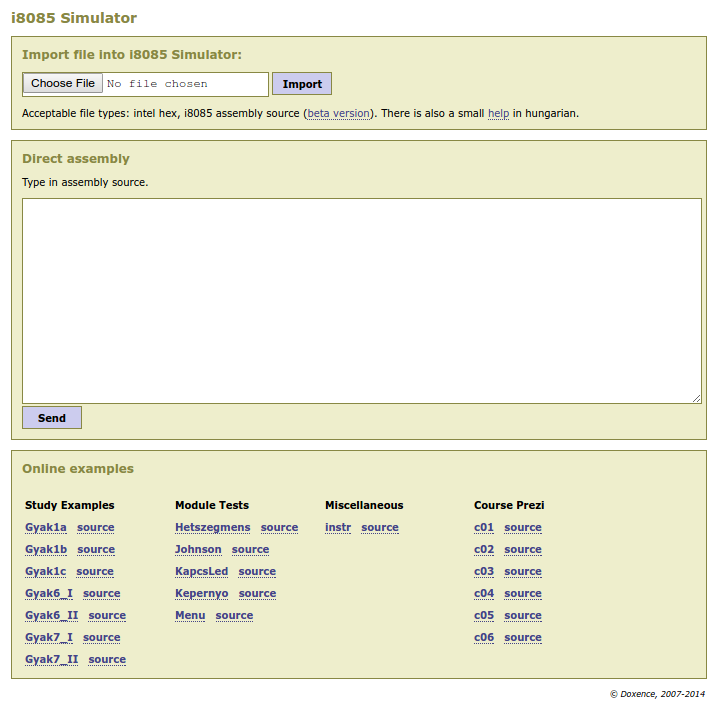
\includegraphics[scale=0.5]{sim.png}

A következő kódot szeretnénk a szimulátorban futtatni:
% asm kód, amit szimulálni szeretnénk
\begin{lstlisting}[frame=single]
ORG 2000h ; 2000h-tol helyezze el a kodot a fordito
LXI H, 2100h ; HL <-- 2100h
MVI M, 11h ; [2100h] = 11h
HLT ; processzor --> HALT allapot
END ; eddig forditson
\end{lstlisting}

\subsubsection{1. lépés: kód beillesztése}
A szimulálandó kódot a Direct assembly ablakba kell írni:

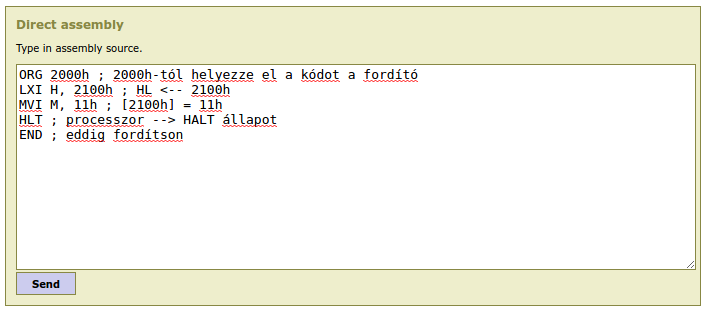
\includegraphics[scale=0.5]{sim_lepes1.png}

Ezután a Send gombra kattintva menjünk tovább, ahol ez fogad minket:

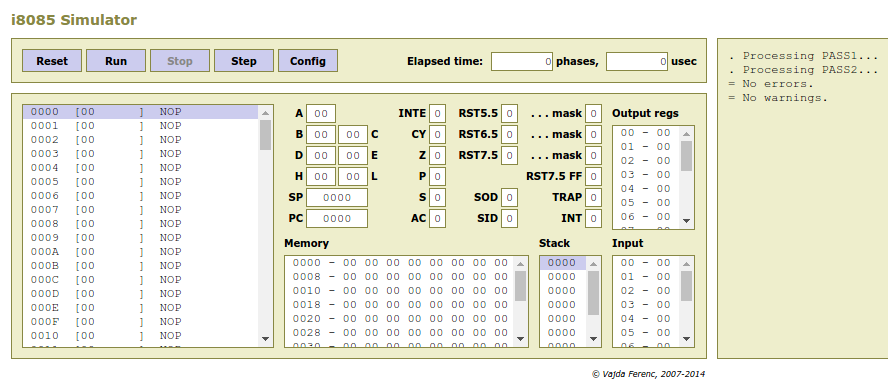
\includegraphics[scale=0.5]{sim_lepes2.png}

\subsubsection{2. lépés: szimuláció beállítása}

Néhány beállítást el kell végeznünk, hogy a megfelelő módon tudjuk nyomon követni a futó kódot.
\begin{enumerate}
	\item Coda Start at: cím, ahova elhelyezzük a kódot (és kattintsunk bele a fehér téglalapba, hogy megjelenjen ott a PC felirat)
	\item Show bus activity: legyen bepipálva
	\item Follow code: legyen bepipálva
\end{enumerate}
Az utolsó 2 opció ahhoz kell, hogy egy szép táblázatos formában jelenítse meg a kód futását és utasításonként haladjon a kód végrehajtása során.
Ezek elvégzése után ezt kell látni:

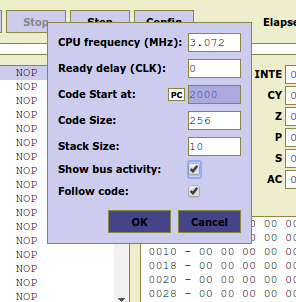
\includegraphics[scale=0.5]{sim_lepes3.png}

Az OK gombra kattintva megjelenik az oldal alján a táblázat fejléce:

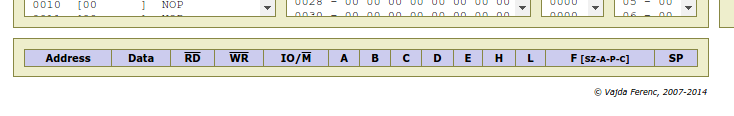
\includegraphics[scale=0.5]{sim_lepes4.png}

A táblázat fejléce:
\begin{enumerate}
	\item Address: milyen címre mutat éppen a PC
	\item Data: milyen adat van ezen a memóriacímen
	\item $\overline{RD}$: olvasás-e a jelenlegi művelet
	\item $\overline{WR}$: írás-e a jelenlegi művelet
	\item $IO/\overline{M}$: a mostani utasítás memória vagy periféria műveletet hajt végre
	\item regiszterek aktuális értékei
	\item F [SZ-A-P-C]: flag-ek aktuális értékei
	\begin{enumerate}
		\item Sign flag: előjel flag
		\item Zero flag: zérus flag
		\item Auxillary carry flag: fél-átvitel flag
		\item Parity flag: paritás flag
		\item Carry flag: átvitel flag
	\end{enumerate}
	\item SP: Stack Pointer aktuális értéke
\end{enumerate}

A PC mezőbe írjuk bele a címet, ahova helyeztük a kódot, jelen példában a 2000h-t:

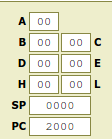
\includegraphics[scale=0.5]{sim_lepes5.png}

Ha be kell állítani a regiszterek kezdőértéket, akkor a megfelelő regiszterek mezőjébe írjuk bele a szükséges értéket.

\subsubsection{3. lépés: kód követése}

A bal oldali ablakban látható, hogy a PC a 2000h-ra mutat, ezt a kék háttérrel jelöli a rendszer (soron következő utasítás).

Ha rámegyünk a Step gombra az oldal tetején, akkor lefuttatja a PC által jelölt utasítást és az oldal alján elhelyezkedő táblázatban megjelenik néhány adat:

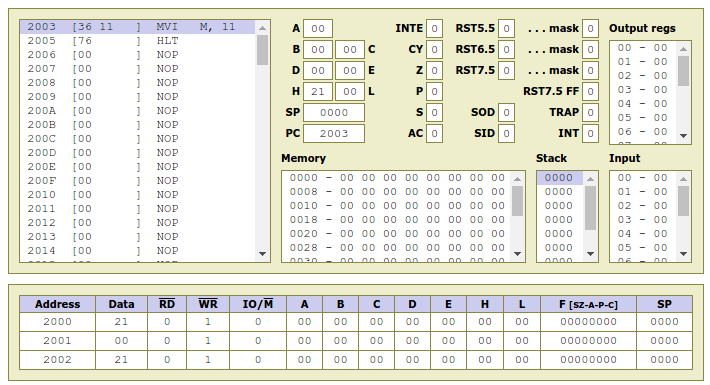
\includegraphics[scale=0.5]{sim_lepes6.png}

Vegyük sorra, hogy mi minden történt:
\begin{enumerate}
	\item A bal oldali fehér ablakban a kék háttér most már a soron következő utasításra mutat (MVI   M, 11), hiszen az előző utasítást már lefuttattuk és tovább lépett.
	\item A táblázatban megjelentek az LXI H, 2100h utasítás során történt dolgok.
	\begin{enumerate}
		\item Mivel a 2000h-ra helyeztük el a kódot, a PC onnan olvassa fel az első adatot. Ott egy LXI utasítás van, ezért az első adat, amit felolvas az az utasítás opkódja.
		\item \colorbox{orange!30}{Ökölszabály: minden utasítás első bájtja az opkódja.}
		\item \colorbox{orange!30}{Opkód: utasítás egyedi azonosító kódja}
		% ami alapján tudja a processzor, hogy milyen fizikai műveleteket kell elvégeznie.
		\item Az LXI utasításhoz 2 dolog tartozik még: a regiszterpár, ahova adatot mozgatunk és maga az adat, amit mozgatunk. A regiszterpár az opkódba van kódolva, ezt a segédletből ki lehet olvasni. A másik paraméter, hogy milyen adatot akarunk elhelyezni a regiszterpárba. 2 bájtos adatot tudunk egy regiszterpárba tenni, ezért ez a 2 bájt az opkódot követő következő 2 címen helyezkedik el.
		\item \colorbox{orange!30}{Little-endian: kisebb címen kisebb helyiérték}
		\item a 2100h számot szeretnénk a HL regiszterekbe tenni, szóval először felolvassuk a 2100h alsó bájtját (00h) a 2001h címről, majd a felső bájtját (21h) a 2002h címről.
		\item \colorbox{orange!30}{Egy utasítás opkódja és a paraméterei címfolytonosan helyekednek el a memóriában}
		\item \colorbox{orange!30}{Címfolytonos: egymást követő memóriacímeken.}
		\item \colorbox{orange!30}{Az opkód és az utasítás paramétereinek beolvasása mind olvasás művelet.}
	\end{enumerate}
	\item A Step-re kattintva lefuttatja a jelenlegi utasítást, ami az MVI M, 11h, majd megjelennek a táblázatban az eközben történtek:
	\begin{enumerate}
		\item Címfolytosan helyezkedik el a kód, szóval a következő címen van az MVI M utasítás opkódja, vagyis a 2003h-n.
		\item Az MVI M utasításhoz tartozik egy paraméter: milyen adatot akarunk elhelyezni az M által mutatott memóriacímre. Ezt az adatot az opkódot követő címről olvassa fel, tehát a 2004h-ról.
		\item Felolvastunk az MVI M, 11h-hoz tartozó minden adatot, szóval el tudjuk ténylegesen végezni az utasítást fizikailag is: elhelyezzük az M által mutatott memóriacímre a 11h-t.
		\item Az M pointer a HL regiszterpár tartalmával jelölt memóriacímre mutat, a HL-ben jelenleg a 2100h van, hiszen az imént tettük bele. Így a 2100h címre írjuk a 11h-t. Ez látszik a táblázatban is. 
		\item Figyeljük meg, hogy a $\overline{WR} = 0$, mert ez egy adat írása egy adott memóriacímre. Az Address oszlopban a 2100h szerepel, hiszen erre a címre írunk adatot. A Data oszlopban a 11h érték szerepel, mert ezt az adatot írjuk oda.
		\item \colorbox{orange!30}{Látható, hogy a H és L oszlopokban a  regiszterpár tartalma az előbb odahelyezett 21h és 00h.}
	\end{enumerate}
	\item Ismételten a Step-re nyomva lefut a HLT utasítás is. A HLT címfolytosan helyezkedik el (hiszen nem volt például ORG direktíva vagy hasonló), tehát a 2005h-n. Az adat csupán az utasítás opkódja, mert ehhez az utasításhoz nem tartozik semmilyen paraméter sem.
	\item Végeztünk, elvileg most megtanultuk használni a szimulátort. Ezek után sok gyakorlással ezekkel az alapokkal már ügyesen fogunk tudni bánni ezzel a hasznos kis segédeszközzel.
\end{enumerate}
\end{document}